\documentclass[tikz,border=16pt]{standalone}
\usepackage{amsmath,amssymb}
\usepackage{tikz}
\usetikzlibrary{arrows.meta, positioning, calc, fit, backgrounds, shapes.geometric}

%% ---- palette ----
\definecolor{cBlue}{RGB}{13,110,200}
\definecolor{cFillBlue}{RGB}{230,242,255}
\definecolor{cGray}{RGB}{95,108,120}
\definecolor{cFillGray}{RGB}{220,222,226}
\definecolor{cOrange}{RGB}{195,95,15}
\definecolor{cFillOrange}{RGB}{255,239,218}
\definecolor{cRed}{RGB}{170,35,35}
\definecolor{cFillRed}{RGB}{255,220,220}
\definecolor{cGreen}{RGB}{30,145,75}
\definecolor{cFillGreen}{RGB}{210,245,225}
\definecolor{cPurple}{RGB}{110,40,180}
\definecolor{cFillPurple}{RGB}{240,228,255}
\definecolor{cTeal}{RGB}{10,130,140}
\definecolor{cFillTeal}{RGB}{215,245,248}
\definecolor{cLegend}{RGB}{250,251,253}

\tikzset{
  actor/.style={rectangle, rounded corners=5pt, draw, minimum width=3.0cm,
                minimum height=0.8cm, font=\bfseries\small, align=center,
                inner sep=5pt, line width=1.4pt},
  actorV/.style={actor, draw=cBlue,   fill=cFillBlue,   text=cBlue},
  actorR/.style={actor, draw=cGreen,  fill=cFillGreen,  text=cGreen},
  cbox/.style={rectangle, rounded corners=4pt, draw, minimum width=3.0cm,
               font=\scriptsize, align=left, inner sep=5pt, line width=1.1pt},
  cboxV/.style={cbox, draw=cBlue,   fill=cFillBlue,   text=cBlue},
  cboxR/.style={cbox, draw=cGreen,  fill=cFillGreen,  text=cGreen},
  cboxP/.style={cbox, draw=cPurple, fill=cFillPurple, text=cPurple},
  cboxO/.style={cbox, draw=cOrange, fill=cFillOrange, text=cOrange},
  cboxAbt/.style={cbox, draw=cRed,  fill=cFillRed,   text=cRed},
  stepbubble/.style={circle, draw=cGray, fill=cFillGray, text=cGray,
                     font=\bfseries\scriptsize, inner sep=2pt, minimum size=0.5cm},
  msgarrow/.style={-{Stealth[length=7pt]}, line width=1.4pt},
  msgarrowB/.style={msgarrow, draw=cBlue},
  msgarrowG/.style={msgarrow, draw=cGreen},
  lifeline/.style={draw=cGray!40, line width=1pt, dashed},
  guard/.style={diamond, shape aspect=2.2, draw=cGray, fill=cFillGray, text=cGray,
                font=\bfseries\scriptsize, inner sep=2pt, align=center},
}

\begin{document}
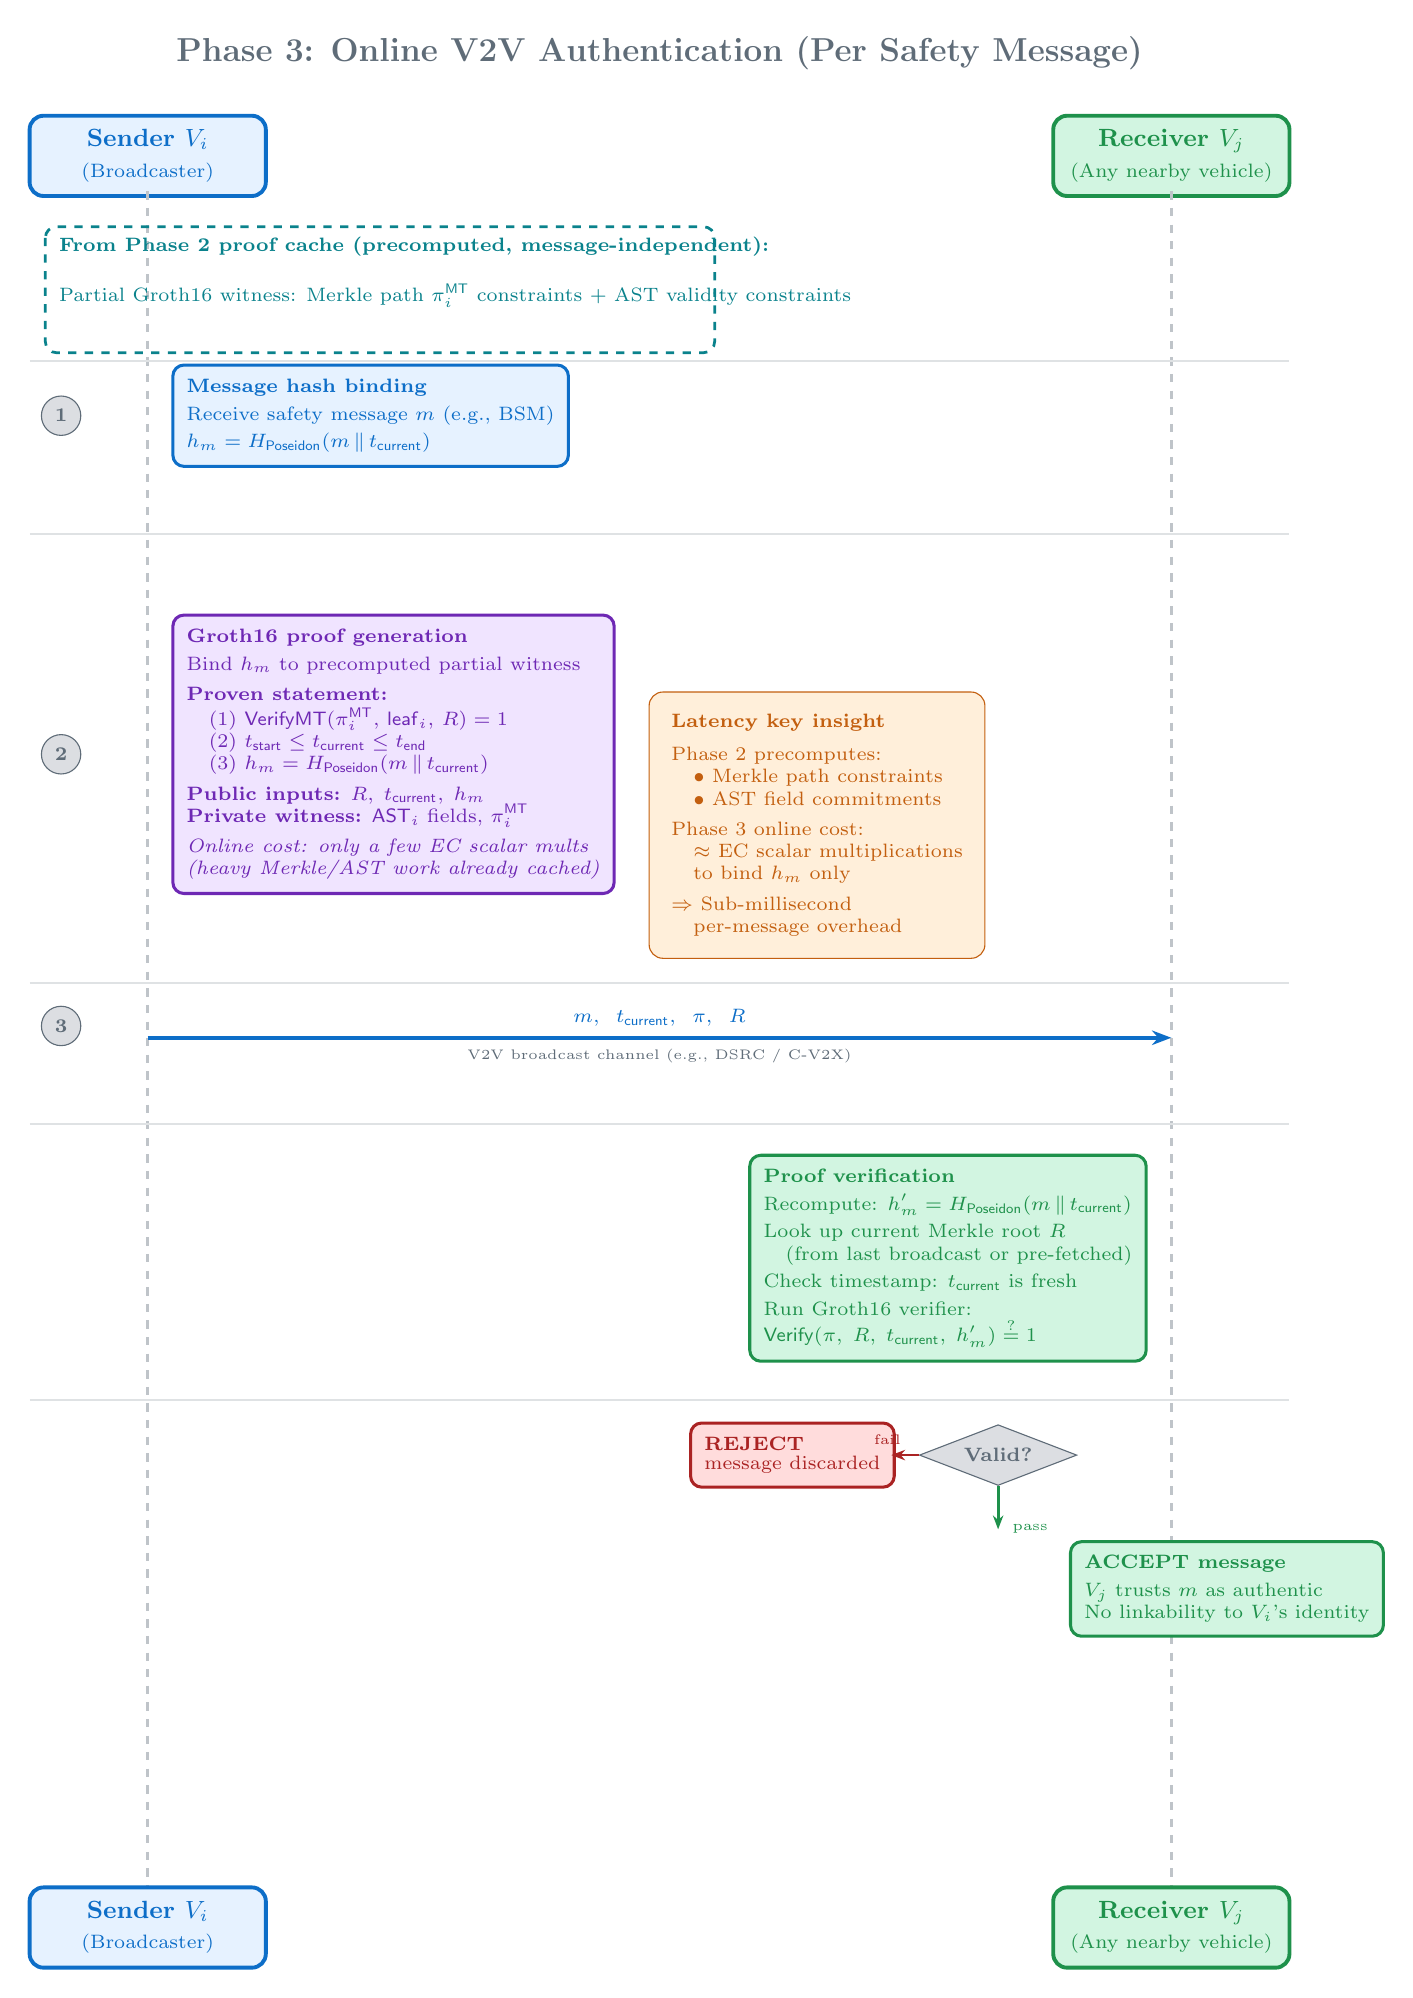
\begin{tikzpicture}

%% ============================================================
%%  ACTOR POSITIONS
%%  Sender Vi at x=0,  Receiver Vj at x=13
%% ============================================================
\def\Vx{0}
\def\Rx{13}

%% ----- Actor headers -----
\node[actorV] (Vi) at (\Vx, 0) {Sender $V_i$\\{\scriptsize\normalfont (Broadcaster)}};
\node[actorR] (Vj) at (\Rx, 0) {Receiver $V_j$\\{\scriptsize\normalfont (Any nearby vehicle)}};

%% ----- Lifelines -----
\draw[lifeline] (\Vx, -0.45) -- (\Vx, -22.5);
\draw[lifeline] (\Rx, -0.45) -- (\Rx, -22.5);

%% ============================================================
%%  PRECONDITION banner (from Phase 2 cache)
%% ============================================================
\draw[cTeal, dashed, line width=1pt, rounded corners=4pt]
  (-1.3, -0.9) rectangle (7.2, -2.5);
\node[cTeal, font=\bfseries\scriptsize, anchor=north west]
  at (-1.25, -0.9) {From Phase 2 proof cache (precomputed, message-independent):};
\node[cTeal, font=\scriptsize, anchor=north west]
  at (-1.25, -1.5) {Partial Groth16 witness: Merkle path $\pi^{\mathsf{MT}}_i$ constraints + AST validity constraints};

%% ============================================================
%%  STEP 1 — Compute message hash  (y = -3.3)
%% ============================================================
\def\ya{-3.3}
\node[stepbubble] at (\Vx-1.1, \ya) {1};
\node[cboxV, anchor=west] at (\Vx+0.3, \ya) {%
  \textbf{Message hash binding}\\[2pt]
  Receive safety message $m$ (e.g., BSM)\\[2pt]
  $h_m = H_{\mathsf{Poseidon}}(m \,\|\, t_{\mathsf{current}})$
};

%% ============================================================
%%  STEP 2 — Generate Groth16 proof  (y = -5.6)
%% ============================================================
\def\yb{-7.6}
\node[stepbubble] at (\Vx-1.1, \yb) {2};
\node[cboxP, anchor=west] at (\Vx+0.3, \yb) {%
  \textbf{Groth16 proof generation}\\[2pt]
  Bind $h_m$ to precomputed partial witness\\[3pt]
  \textbf{Proven statement:}\\[1pt]
  \quad (1)~$\mathsf{VerifyMT}(\pi^{\mathsf{MT}}_i,\, \mathsf{leaf}_i,\, R) = 1$\\
  \quad (2)~$t_{\mathsf{start}} \leq t_{\mathsf{current}} \leq t_{\mathsf{end}}$\\
  \quad (3)~$h_m = H_{\mathsf{Poseidon}}(m \,\|\, t_{\mathsf{current}})$\\[3pt]
  \textbf{Public inputs:} $R,\; t_{\mathsf{current}},\; h_m$\\
  \textbf{Private witness:} $\mathsf{AST}_i$ fields, $\pi^{\mathsf{MT}}_i$\\[3pt]
  \textit{Online cost: only a few EC scalar mults}\\
  \textit{(heavy Merkle/AST work already cached)}
};

%% ============================================================
%%  STEP 3 — Vi broadcasts over V2V channel  (y = -11.2)
%% ============================================================
\def\yc{-11.2}
\node[stepbubble] at (\Vx-1.1, \yc+0.15) {3};

\draw[msgarrowB] (\Vx, \yc) -- (\Rx, \yc)
  node[midway, above, font=\scriptsize\bfseries, text=cBlue]
    {$m,\;\; t_{\mathsf{current}},\;\; \pi,\;\; R$}
  node[midway, below, font=\tiny, text=cGray]
    {V2V broadcast channel (e.g., DSRC / C-V2X)};

%% ============================================================
%%  RECEIVER SIDE — Vj verification  (y = -13.0)
%% ============================================================
\def\yd{-14.0}
\node[cboxR, anchor=east] at (\Rx-0.3, \yd) {%
  \textbf{Proof verification}\\[2pt]
  Recompute: $h_m' = H_{\mathsf{Poseidon}}(m \,\|\, t_{\mathsf{current}})$\\[2pt]
  Look up current Merkle root $R$ \\
  \quad (from last broadcast or pre-fetched)\\[2pt]
  Check timestamp: $t_{\mathsf{current}}$ is fresh\\[2pt]
  Run Groth16 verifier:\\
  $\mathsf{Verify}(\pi,\; R,\; t_{\mathsf{current}},\; h_m') \stackrel{?}{=} 1$
};

%% guard diamond
\node[guard, minimum width=2.0cm, minimum height=0.7cm]
  (guard1) at (\Rx-2.2, -16.5) {Valid?};

%% pass branch
\node[cboxR, anchor=west, minimum width=2.5cm,
      draw=cGreen, fill=cFillGreen, text=cGreen]
  at (\Rx-1.3, -18.2) {%
    \textbf{ACCEPT message}\\[2pt]
    $V_j$ trusts $m$ as authentic\\
    No linkability to $V_i$'s identity
  };
\draw[-{Stealth[length=5pt]}, cGreen, line width=1pt]
  (guard1.south) -- ++(0,-0.55)
  node[right, font=\tiny, text=cGreen, xshift=0.05cm] {pass};

%% fail branch
\node[cboxAbt, anchor=east, minimum width=2.5cm]
  at (\Rx-3.5, -16.5) {%
    \textbf{REJECT}\\[-1pt]
    message discarded
  };
\draw[-{Stealth[length=5pt]}, cRed, line width=1pt]
  (guard1.west) -- ++(-0.35,0)
  node[above, font=\tiny, text=cRed, xshift=-0.05cm] {fail};

%% ============================================================
%%  Key insight callout box
%% ============================================================
\node[draw=cOrange, fill=cFillOrange, rounded corners=5pt,
      font=\scriptsize, align=left, inner sep=8pt, text=cOrange,
      minimum width=4.2cm]
  at (8.5, -8.5) {%
    \textbf{Latency key insight}\\[4pt]
    Phase 2 precomputes:\\
    \quad $\bullet$~Merkle path constraints\\
    \quad $\bullet$~AST field commitments\\[3pt]
    Phase 3 online cost:\\
    \quad $\approx$ EC scalar multiplications\\
    \quad to bind $h_m$ only\\[3pt]
    $\Rightarrow$ Sub-millisecond\\
    \quad per-message overhead
};

%% ============================================================
%%  TITLE
%% ============================================================
\node[font=\bfseries\large, text=cGray] at (6.5, 1.3)
  {Phase 3: Online V2V Authentication (Per Safety Message)};

%% ============================================================
%%  Horizontal separators
%% ============================================================
\foreach \yy in {-2.6, -4.8, -10.5, -12.3, -15.8} {
  \draw[cGray!20, line width=0.7pt] (-1.5, \yy) -- (14.5, \yy);
}

%% ============================================================
%%  Actor footers
%% ============================================================
\node[actorV] at (\Vx, -22.5) {Sender $V_i$\\{\scriptsize\normalfont (Broadcaster)}};
\node[actorR] at (\Rx, -22.5) {Receiver $V_j$\\{\scriptsize\normalfont (Any nearby vehicle)}};

\end{tikzpicture}
\end{document}